\documentclass[12pt]{report}

\usepackage{graphicx, color}
\usepackage[utf8]{inputenc}
\usepackage[english]{babel}
\usepackage[a4paper,margin=2cm]{geometry}
\usepackage[maxbibnames=99]{biblatex}
\addbibresource{main.bib}
\usepackage{booktabs}
\usepackage{hyperref}
\usepackage{breakurl}
\hypersetup{
    pdftitle={Drift detection on embeddings},
    pdfauthor={Theofilos Papapanagiotou},
    pdfsubject={Drift detection on contextual embeddings},
    baseurl={https://doi.org/10.5281/zenodo.5625651},
    pdfdisplaydoctitle={true},
    pdffitwindow={false},
    pdfkeywords={machine learning, monitoring, contextual embeddings, language models},
    pdfprintscaling={None},
    pdfpagelayout={SinglePage},
    setpagesize={true},
}
\usepackage{hyperxmp}

\begin{document}





\begin{titlepage}



\newcommand{\HRule}{\rule{\linewidth}{0.5mm}}
\center

 

%----------------------------------------------------------------------------------------

%	HEADING SECTIONS

%----------------------------------------------------------------------------------------


\textsc{\Large MSc Artificial Intelligence}\\[0.2cm]

\textsc{\Large Master Thesis}\\[0.5cm] 



%----------------------------------------------------------------------------------------

%	TITLE SECTION

%----------------------------------------------------------------------------------------



\HRule \\[0.4cm]

{ \huge \bfseries Drift detection on embeddings}\\[0.4cm]

\HRule \\[0.5cm]

 

%----------------------------------------------------------------------------------------

%	AUTHOR SECTION

%----------------------------------------------------------------------------------------



by\\[0.2cm]

\textsc{\Large Theofilos Papapanagiotou}\\[0.2cm]

{11903406}\\[1cm]





%----------------------------------------------------------------------------------------

%	DATE SECTION

%----------------------------------------------------------------------------------------



{\Large \today}\\[1cm]



42 Credits\\ %

November 2021 - June 2022\\[1cm]%



%----------------------------------------------------------------------------------------

%	COMMITTEE SECTION

%----------------------------------------------------------------------------------------

\begin{minipage}[t]{0.4\textwidth}

\begin{flushleft} \large

\emph{Supervisor:} \\

\textsc{dr. ing. Sebastian Schelter }\\

\end{flushleft}

\end{minipage}

~

\begin{minipage}[t]{0.4\textwidth}

\begin{flushright} \large

\emph{Examiner:} \\

\textsc{dr. ing. Sebastian Schelter }\\

\vspace{0.5cm}

\emph{Second reader:} \\

\textsc{ing. Barrie Kersbergen}\\

\end{flushright}

\end{minipage}\\[2cm]



%----------------------------------------------------------------------------------------

%	LOGO SECTION

%----------------------------------------------------------------------------------------




\includegraphics[width=10cm]{uvalogo_regular_p_nl.eps}

 

%----------------------------------------------------------------------------------------



\vfill

\end{titlepage}

\pagenumbering{roman}

\tableofcontents

\begin{abstract}
%We might hope that when faced with unexpected inputs, well-designed software systems would fire off warnings. Machine learning (ML) systems, however, which depend strongly on properties of their inputs (e.g. the i.i.d. assumption), tend to fail silently. This paper explores the problem of building ML systems that fail loudly, investigating methods for detecting dataset shift, identifying exemplars that most typify the shift, and quantifying shift malignancy. We focus on several datasets and various perturbations to both covariates and label distributions with varying magnitudes and fractions of data affected. Interestingly, we show that across the dataset shifts that we explore, a two-sample-testing-based approach, using pre-trained classifiers for dimensionality reduction, performs best. Moreover, we demonstrate that domain-discriminating approaches tend to be helpful for characterizing shifts qualitatively and determining if they are harmful.

%domain: contextual embedding from language model
%task: detect drift
%method: empirical study

% drift detection = compare distributions
%
%p(x)=q(x') vs p(x)!=q(x')
%
%comparing distributions of single or small dimentional vectors is simple
%multidiemensional vectors such as the contectual embeddings of the modern LLMs, are more difficult
Language models produce multidimensional vectors, but the context of the embedding is not known.
Storing the embeddings in a platform also requires advanced monitoring capabilities to detect data shifts.
Drift detection in the domain of contextual embeddings is a challenging task, as it requires a large number of data points to be compared.
This thesis is an empirical study of the problem of detecting data shifts in the domain of contextual embeddings.
We see that a pre-trained classifier for dimensionality reduction can be used to detect data shifts, and performs better than traditional methods like MMD, KS and LSDD.
We also analyse the problem of scaling such a solution and discuss the implications of implementing such a system in a ML platform.

\end{abstract}

\pagenumbering{arabic}

\chapter{Introduction}
%%-----Failing start
%Software systems employing deep neural networks are now applied widely in industry, powering the vision systems in social networks [47] and self-driving cars [5], providing assistance to radiologists [24], underpinning recommendation engines used by online platforms [9, 12], enabling the bestperforming commercial speech recognition software [14, 21], and automating translation between languages [50].
%In each of these systems, predictive models are integrated into conventional humaninteracting software systems, leveraging their predictions to drive consequential decisions.
%The reliable functioning of software depends crucially on tests.
%Many classic software bugs can be caught when software is compiled, e.g. that a function receives input of the wrong type, while other problems are detected only at run-time, triggering warnings or exceptions.
%In the worst case, if the errors are never caught, software may behave incorrectly without alerting anyone to the problem.
%Unfortunately, software systems based on machine learning are notoriously hard to test and maintain [42].
%Despite their power, modern machine learning models are brittle.
%Seemingly subtle changes in the data distribution can destroy the performance of otherwise state-of-the-art classifiers, a phenomenon exemplified by adversarial examples [51, 57].
%When decisions are made under uncertainty, even shifts in the label distribution can significantly compromise accuracy [29, 56].
%Unfortunately, in practice, ML pipelines rarely inspect incoming data for signs of distribution shift.
%Moreover, best practices for detecting shift in high-dimensional real-world data have not yet been established2.
%In this paper, we investigate methods for detecting and characterizing distribution shift, with the hope of removing a critical stumbling block obstructing the safe and responsible deployment of machine learning in high-stakes applications.
%Faced with distribution shift, our goals are three-fold:
%(i) detect when distribution shift occurs from as few examples as possible;
%(ii) characterize the shift, e.g. by identifying those samples from the test set that appear over-represented in the target data; and
%(iii) provide some guidance on whether the shift is harmful or not.
%As part of this paper we principally focus on goal
%(i) and explore preliminary approaches to (ii) and (iii).
%We investigate shift detection through the lens of statistical two-sample testing.
%We wish to test the equivalence of the source distribution p (from which training data is sampled) and target distribution q (from which real-world data is sampled).
%For simple univariate distributions, such hypothesis testing is a mature science.
%However, best practices for two sample tests with high-dimensional (e.g. image) data remain an open question.
%While off-the-shelf methods for kernel-based multivariate two-sample tests are appealing, they scale badly with dataset size and their statistical power is known to decay badly with high ambient dimension [37].
%Recently, Lipton et al. [29] presented results for a method called black box shift detection (BBSD), showing that if one possesses an off-the-shelf label classifier f with an invertible confusion matrix, then detecting that the source distribution p differs from the target distribution q requires only detecting that p(f (x)) 6= q(f (x)).
%Building on their idea of combining black-box dimensionality reduction with subsequent two-sample testing, we explore a range of dimensionality-reduction techniques and compare them under a wide variety of shifts (Figure 1 illustrates our general framework).
%We show (empirically) that BBSD works surprisingly well under a broad set of shifts, even when the label shift assumption is not met.
%Furthermore, we provide an empirical analysis on the performance of domain-discriminating classifier-based approaches (i.e. classifiers explicitly trained to discriminate between source and target samples), which has so far not been characterized for the complex high-dimensional data distributions on which modern machine learning is routinely deployed.
%%-----Failing end

Machine learning systems are used in the industry to learn users' dietary habits, entertainment preferences, financial behaviour, etc.
By doing so, they power the most innovative products which take advantage of that rich, ever-changing information.
The evolution of data processing in order to better encode the underlying information, is a key driver for the success of these systems.
The transformation of the data to features is a key part of the modeling process.
But such models, are not always robust to the presence of distribution shift in the data.

Storing the features in a dedicated system such as a feature store, helps decoupling the generation of the features from the consumption \cite{MachineLearningDesign}.
Data analysts with domain expertise generate features from the data.
Data scientists consume these features to build models, focusing on the modeling activity.

Today, language models (LMs) and large language models (LLMs) are used to extract embeddings from text data.
They are used by downstream tasks to perform prediction actions on new data.
The most common activity over these embeddings is the similarity search, to find the nearest neighbors of a given embedding.
The utilization of an embeddings store next to a feature store brings a significant advantage to development process \cite{orrManagingMLPipelines2021}.
By using a vector database as an embedding store, we can avoid the need to load the full set of embeddings into memory.
Essentially we offload the task of the search to a dedicated system \cite{wangMilvusPurposeBuiltVector2021} \cite{weiAnalyticDBVHybridAnalytical2020}.

Continuous model training pipelines make use of signals observed during inference time, to trigger the retraining of models \cite{baylorContinuousTrainingProduction2019}.
Such signals are produced by monitoring techniques \cite{papapanagiotouModelMonitoring2021} that understand the changes in the data quality \cite{schelterAutomatingLargescaleData2018a} and eventually the degradation of the model's performance.
% TODO drift detection sits next to the feature&embeddings store as a monitoring mechanism
Drift detection is a common technique, used to detect the presence of distribution shift in the data.

Common drift detection methods rely on dimensionality reduction techniques on the features of the data, seeing success in the modalities of image and tabular data.
In the case of text data though detecting shift in the words or the sentences is not effective, as they do not represent the semantics of the input \cite{ltdAlibidetectDocumentationb}.
The introduction of LMs and LLMs brings the heavy use of the contextual embdeddings.
These embeddings are vectors of floats, extracted by the last layers of pre-trained models, sometimes fine-tuned to improve the performance of the model on a particular domain.
The detection takes place on the embeddings, and not on the raw input data.

In this thesis, we study empirically the use of drift detectors on such contextual embeddings, extracted by modern LMs.
Reviewing the literature, we see that there has been significant studies \cite{rabanserFailingLoudlyEmpirical2019a} in other modalities.
We also see that detecting distribution shifts in embeddings is not a popular topic in the literature.
We explore the mechanics of shift detectors such as Maximum Mean Discrepancy (MMD), Kolmogorov-Smirnov (KS), Least Squares Density Difference (LSDD) and a pre-trained classifier (DistilBERT).
In the experiment section we evaluate the performance of these methods on the embeddings of the text data, measured on the original and drifted test sets.
We use the notion of distance as well as the runtime to discuss the results of the experiment and their applicability to production use-cases.
We see that dimensionality reduction with subsequent two-sample testing, which is a common preprocessing task on the other modalities, is not effective the case of embeddings of text data.
We also see that the use of a pre-trained classifier is not efficient for online drift detection.

%classifier: dimensionality reduction with subsequent two-sample testing
%
%Dimension reduction is a common preprocessing task (e.g. for covariate drift detection on tabular or image data),
%but some modalities of data (e.g. text and graph data) require other forms of preprocessing in order for drift detection
%to be performed effectively.


\chapter{Related work}

% Given just one example from the test data, our problem simplifies to anomaly detection, surveyed thoroughly by Chandola et al. [8] and Markou and Singh [33].
% Popular approaches to anomaly detection include density estimation [6], margin-based approaches such as the one-class SVM [40], and the tree-based isolation forest method due to [30].
% Recently, also GANs have been explored for this task [39].
% Given simple streams of data arriving in a time-dependent fashion where the signal is piece-wise stationary with abrupt changes, this is the classic time series problem of change point detection, surveyed comprehensively by Truong et al. [52].
% An extensive literature addresses dataset shift in the context of domain adaptation.
% Owing to the impossibility of correcting for shift absent assumptions [3], these papers often assume either covariate shift q(x, y) = q(x)p(y|x) [15, 45, 49] or label shift q(x, y) = q(y)p(x|y) [7, 29, 38, 48, 56].
% Sch ̈ olkopf et al. [41] provides a unifying view of these shifts, associating assumed invariances with the corresponding causal assumptions.
% Several recent papers have proposed outlier detection mechanisms dubbing the task out-ofdistribution (OOD) sample detection.
% Hendrycks and Gimpel [19] proposes to threshold the maximum softmax entry of a neural network classifier which already contains a relevant signal.
% Liang et al. [28] and Lee et al. [26] extend this idea by either adding temperature scaling and adversarial like perturbations on the input or by explicitly adapting the loss to aid OOD detection.
% Choi and Jang [10] and Shalev et al. [44] employ model ensembling to further improve detection reliability.
% Alemi et al. [2] motivate use of the variational information bottleneck.
% Hendrycks et al. [20] expose the model to OOD samples, exploring heuristics for discriminating between in-distribution and out-of-distribution samples.
% Shafaei et al. [43] survey numerous OOD detection techniques.

Tsymbal et al \cite{tsymbalProblemConceptDrift} describes that two kinds of concept drift that may occur in the real world are normally distinguished in the literature as (1) sudden (abrupt, instantaneous) and (2) gradual concept drift.
Lu et al \cite{luLearningConceptDrift2018} describe a general framework for concept drift detection.
Gama et al \cite{gamajoaoSurveyConceptDrift2014} introduce the concept drift adaptation and present the state of the art techniques and a collection of benchmarks.

Investigation of methods for detecting dataset shift on the modality of computer vision show that the best performance is achieved by the two-sample testing with pre-trained classifiers for dimensionality reduction \cite{rabanserFailingLoudlyEmpirical2019a}.
Feldhans et al \cite{feldhansDriftDetectionText2021} empirically compare drift detectors on document embeddings on two benchmarking datasets with varying amounts of drift. Their results show that multivariate drift detectors based on the KTS Test and LSDD outperform univariate drift detectors based on the KS Test.

Douadi et al \cite{bouadiAdvancesIntelligentData2022} compare different types of dissimilarity estimators and metrics theoretically and empirically and investigate the relevance of the single metric components.
Kubler et al \cite{kublerAutoMLTwoSampleTest2022} uses an AutoML two-sample test and achieves competitive performance on a diverse distribution shift benchmark as well as on challenging two-sample testing problems.
Zhao et al \cite{zhaoComparingDistributionsMeasuring2022} proposes a general framework that generalizes the JensenShannon divergence and the maximum mean discrepancy family.
Cobb and Looveren explore context-aware drift detection \cite{cobbContextAwareDriftDetection2022} and additionally contribute the alibi-detect library \cite{vanlooverenAlibiDetectAlgorithms2022}

\chapter{Drift detection techniques}

To formalize the problem, our training dataset is processed through the pretrained model and the extracted embeddings form the dataset \(x\) with a distribution \(p(x)\).
Our test dataset is processed with the same way and produce the dataset \(x'\) with a distribution \(q(x')\).
We want to determine if \(p(x)=q(x')\).
In hypothesis testing, the null hypothesis would be \(H_0: p(x)=q(x')\) and the alternate hypothesis \(H_A: p(x) \neq q(x') \).
Unlike other experiments \cite{rabanserFailingLoudlyEmpirical2019a}, the datasets \(x\) and \(x'\) are high-dimensional latent space representations of the text data.

\begin{figure}[h]
    \centering
    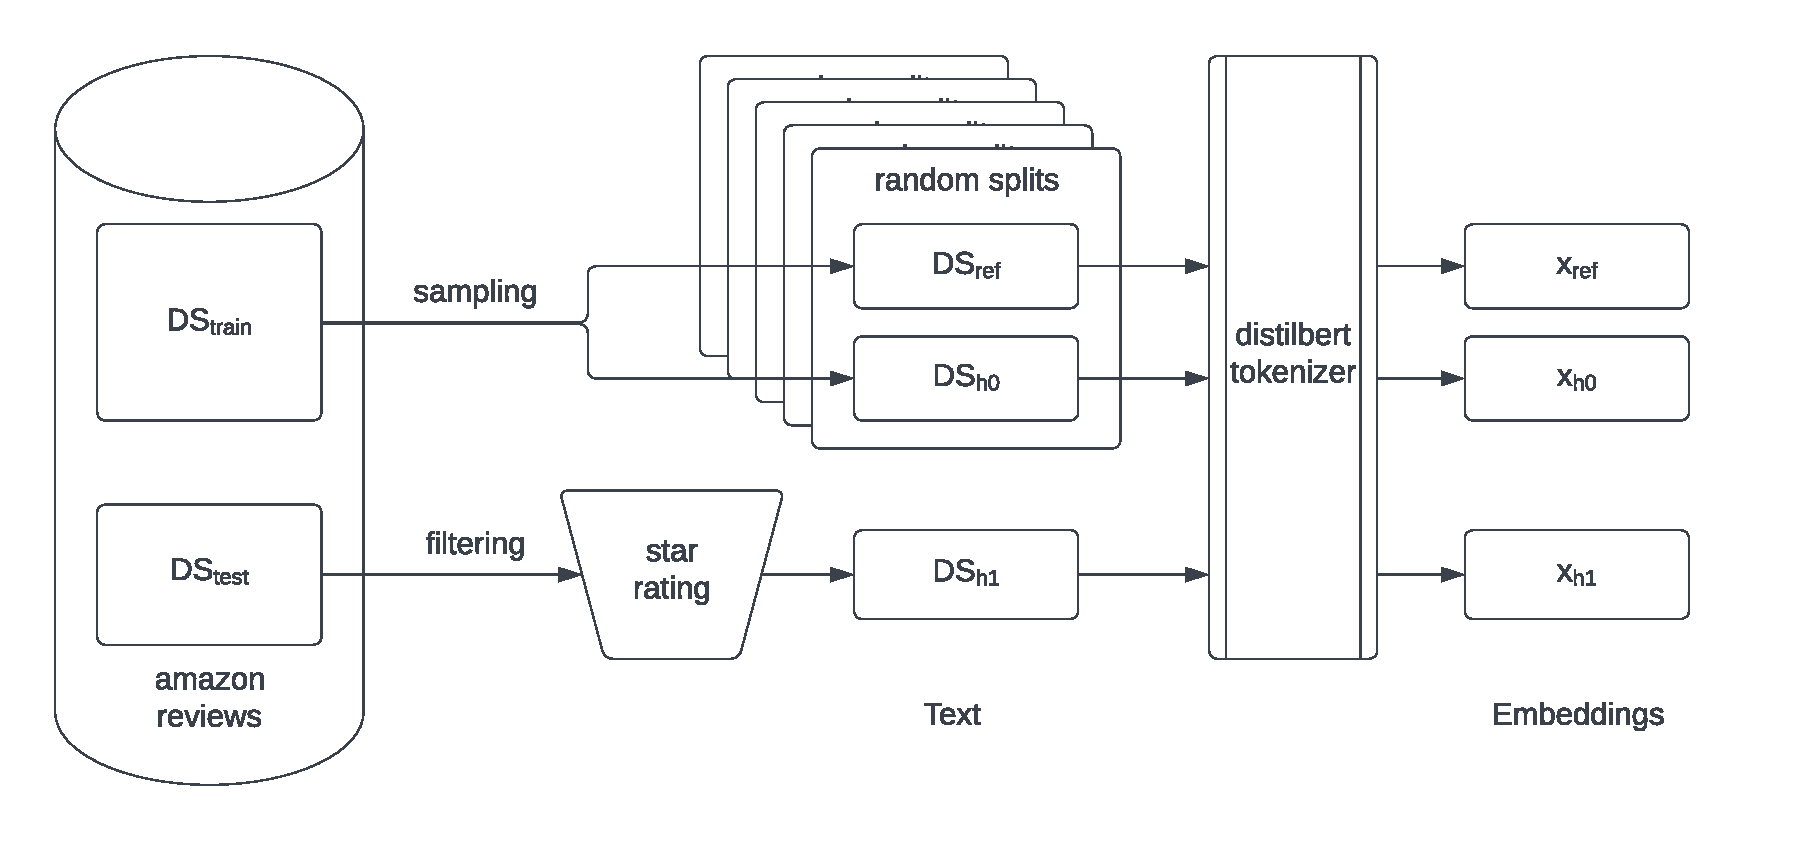
\includegraphics[width=0.7\linewidth]{images/data_split}
    \caption{Dataset split into reference and tests subsets before the detection of drift}
    \label{fig:data_split}
\end{figure}

As we randomly sample \(DS_{ref}\) and \(DS_{h0}\) from the dataset and subsequently generate the embedings \(x_{ref}\) and \(x_{h0}\), we do not expect them to have an identical distribution, but close enough to be used for the null hypothesis test.
On the other hand, we induce drift in the \(DS_{h1}\) dataset by filtering from the test subset the text of a particular use behaviour, reflected into the star rating feature of the dataset.
The embeddings \(x_{h1}\) should be further away in terms of distance from the embeddings of \(x_{ref}\) and \(x_{h0}\) and therefore be used for the alternate hypothesis test.



% Given labeled data {(x1, y1), ..., (xn, yn)} ∼ p and unlabeled data {x′1, ..., x′m} ∼ q, our task is to determine whether p(x) equals q(x′).
% Formally, H0 : p(x) = q(x′) vs HA : p(x) 6= q(x′).
% Chiefly, we explore the following design considerations:
% (i) what representation to run the test on;
% (ii) which two-sample test to run;
% (iii) when the representation is multidimensional;
% whether to run multivariate or multiple univariate two-sample tests; and
% (iv) how to combine their results.

% 3.1 Dimensionality Reduction
% We now introduce the multiple dimensionality reduction (DR) techniques that we compare visa-vis their effectiveness in shift detection (in concert with two-sample testing).
% Note that absent assumptions on the data, these mappings, which reduce the data dimensionality from D to K (with K  D), are in general surjective, with many inputs mapping to the same output.
% Thus, it is trivial to construct pathological cases where the distribution of inputs shifts while the distribution of lowdimensional latent representations remains fixed, yielding false negatives.
% However, we speculate that in a non-adversarial setting, such shifts may be exceedingly unlikely.
% Thus our approach is (i) empirically motivated; and (ii) not put forth as a defense against worst-case adversarial attacks.
% No Reduction (NoRed ): To justify the use of any DR technique, our default baseline is to run tests on the original raw features.
% Principal Components Analysis (PCA ):% Principal components analysis is a standard tool that finds an optimal orthogonal transformation matrix R such that points are linearly uncorrelated after transformation.
% This transformation is learned in such a way that the first principal component accounts for as much of the variability in the dataset as possible, and that each succeeding principal component captures as much of the remaining variance as possible subject to the constraint that it be orthogonal to the preceding components.
% Formally, we wish to learn R given X under the mentioned constraints such that ˆ X = XR yields a more compact data representation.
% Sparse Random Projection (SRP ): Since computing the optimal transformation might be expensive in high dimensions, random projections are a popular DR technique which trade a controlled amount of accuracy for faster processing times.
% Specifically, we make use of sparse random projections, a more memory- and computationally-efficient modification of standard Gaussian random projections.
% Formally, we generate a random projection matrix R and use it to reduce the dimensionality of a given data matrix X, such that ˆ X = XR.
% The elements of R are generated using the following rule set [1, 27]: Rij =      + √v K with probability 1 2v 0 with probability 1 − 1 v where v = 1 √D . − √v K with probability 1 2v (1)
% Autoencoders (TAE and UAE ): We compare the above-mentioned linear models to non-linear reduced-dimension representations using both trained (TAE) and untrained autoencoders (UAE).
% Formally, an autoencoder consists of an encoder function φ : X → H and a decoder function ψ : H → X where the latent space H has lower dimensionality than the input space X .
% As part of the training process, both the encoding function φ and the decoding function ψ are learned jointly to reduce the reconstruction loss: φ, ψ = arg minφ,ψ ‖X − (ψ ◦ φ)X‖2. Label Classifiers (BBSDs / and BBSDh .):
% Motivated by recent results achieved by black box shift detection (BBSD) [29], we also propose to use the outputs of a (deep network) label classifier trained on source data as our dimensionality-reduced representation.
% We explore variants using either the softmax outputs (BBSDs) or the hard-thresholded predictions (BBSDh) for subsequent two-sample testing. Since both variants provide differently sized output (with BBSDs providing an entire softmax vector and BBSDh providing a one-dimensional class prediction), different statistical tests are carried out on these representations.
% Domain Classifier (Classif ×): Here, we attempt to detect shift by explicitly training a domain classifier to discriminate between data from source and target domains.
% To this end, we partition both the source data and target data into two halves, using the first to train a domain classifier to distinguish source (class 0) from target (class 1) data.
% We then apply this model to the second half and subsequently conduct a significance test to determine if the classifier’s performance is statistically different from random chance.

% 3.2 Statistical Hypothesis Testing
% The DR techniques each yield a representation, either uni- or multi-dimensional, and either continuous or discrete, depending on the method.
% The next step is to choose a suitable statistical hypothesis test for each of these representations.
% Multivariate Kernel Two-Sample Tests:
% Maximum Mean Discrepancy (MMD): For all multidimensional representations, we evaluate the Maximum Mean Discrepancy [16], a popular kernelbased technique for multivariate two-sample testing.
% MMD allows us to distinguish between two probability distributions p and q based on the mean embeddings μp and μq of the distributions in a reproducing kernel Hilbert space F, formally MMD(F , p, q) = ||μp − μq||2F . (2)
% Given samples from both distributions, we can calculate an unbiased estimate of the squared MMD statistic as follows MMD2 = 1 m2 − m m ∑ i=1 m ∑ j6=i κ(xi, xj) + 1 n2 − n n ∑ i=1 n ∑ j6=i κ(x′ i, x′ j) − 2 mn m ∑ i=1 n ∑ j=1 κ(xi, x′ j) (3) where we use a squared exponential kernel κ(x,  ̃ x) = e− 1 σ ‖x− ̃ x‖2 and set σ to the median distance between points in the aggregate sample over p and q [16].
% A p-value can then be obtained by carrying out a permutation test on the resulting kernel matrix.
% Multiple Univariate Testing:
% Kolmogorov-Smirnov (KS) Test + Bonferroni Correction: As a simple baseline alternative to MMD, we consider the approach consisting of testing each of the K dimensions separately (instead testing over all dimensions jointly).
% Here, for continuous data, we adopt the Kolmogorov-Smirnov (KS) test, a non-parametric test whose statistic is calculated by computing the largest difference Z of the cumulative density functions (CDFs) over all values z as follows Z = sup z |Fp(z) − Fq(z)| (4) where Fp and Fq are the empirical CDFs of the source and target data, respectively.
% Under the null hypothesis, Z follows the Kolmogorov distribution.
% Since we carry out a KS test on each of the K components, we must subsequently combine the pvalues from each test, raising the issue of multiple hypothesis testing.
% As we cannot make strong assumptions about the (in)dependence among the tests, we rely on a conservative aggregation method, notably the Bonferroni correction [4], which rejects the null hypothesis if the minimum p-value among all tests is less than α/K (where α is the significance level of the test).
% While several less conservative aggregations methods have been proposed [18, 32, 46, 53, 55], they typically require assumptions on the dependencies among the tests.
% Categorical Testing: Chi-Squared Test: For the hard-thresholded label classifier (BBSDh), we employ Pearson’s chi-squared test, a parametric tests designed to evaluate whether the frequency distribution of certain events observed in a sample is consistent with a particular theoretical distribution.
% Specifically, we use a test of homogeneity between the class distributions (expressed in a contingency table) of source and target data.
% The testing problem can be formalized as follows: Given a contingency table with 2 rows (one for absolute source and one for absolute target class frequencies) and C columns (one for each of the C-many classes) containing observed counts Oij, the expected frequency under the independence hypothesis for a particular cell is Eij = Nsumpi•p•j with Nsum being the sum of all cells in the table, pi• = Oi• Nsum = ∑C j=1 Oij Nsum being the fraction of row totals, and p•j = O•j Nsum = ∑2 i=1 Oij Nsum being the fraction of column totals.
% The relevant test statistic X2 can be computed as X2 = 2 ∑ i=1 C ∑ j=1 (Oij − Eij )2 Eij (5) which, under the null hypothesis, follows a chi-squared distribution with C − 1 degrees of freedom: X2 ∼ χ2 C−1.
% Binomial Testing: For the domain classifier, we simply compare its accuracy (acc) on held-out data to random chance via a binomial test.
% Formally, we set up a testing problem H0 : acc = 0.5 vs HA : acc 6= 0.5.
% Under the null hypothesis, the accuracy of the classifier follows a binomial distribution: acc ∼ Bin(Nhold, 0.5), where Nhold corresponds to the number of held-out samples.

% 3.3 Obtaining Most Anomalous Samples
% As our detection framework does not detect outliers but rather aims at capturing top-level shift dynamics, it is not possible for us to decide whether any given sample is in- or out-of-distribution.
% However, we can still provide an indication of what typical samples from the shifted distribution look like by harnessing domain assignments from the domain classifier.
% Specifically, we can identify the exemplars which the classifier was most confident in assigning to the target domain.
% Since the domain classifier assigns class-assignment confidence scores to each incoming sample via the softmax-layer at its output, it is easy to create a ranking of samples that are most confidently believed to come from the target domain (or, alternatively, from the source domain).
% Hence, whenever the binomial test signals a statistically significant accuracy deviation from chance, we can use use the domain classifier to obtain the most anomalous samples and present them to the user.
% In contrast to the domain classifier, the other shift detectors do not base their shift detection potential on explicitly deciding which domain a single sample belongs to, instead comparing entire distributions against each other.
% While we did explore initial ideas on identifying samples which if removed would lead to a large increase in the overall p-value, the results we obtained were unremarkable.

% 3.4 Determining the Malignancy of a Shift
% Theoretically, absent further assumptions, distribution shifts can cause arbitrarily severe degradation in performance.
% However, in practice distributions shift constantly, and often these changes are benign.
% Practitioners should therefore be interested in distinguishing malignant shifts that damage predictive performance from benign shifts that negligibly impact performance.
% Although prediction quality can be assessed easily on source data on which the black-box model f was trained, we are not able compute the target error directly without labels.
% We therefore explore a heuristic method for approximating the target performance by making use of the domain classifier’s class assignments as follows:
% Given access to a labeling function that can correctly label samples, we can feed in those examples predicted by the domain classifier as likely to come from the target domain.
% We can then compare these (true) labels to the labels returned by the black box model f by feeding it the same anomalous samples.
% If our model is inaccurate on these examples (where the exact threshold can be user-specified to account for varying sensitivities to accuracy drops), then we ought to be concerned that the shift is malignant.
% Put simply, we suggest evaluating the accuracy of our models on precisely those examples which are most confidently assigned to the target domain

\section{Kolmogorov-Smirnov (KS) Test}
The Kolmogorov-Smirnov (KS) test is a non-parametric test for the null hypothesis that two distributions are identical.
The aim of this test is to compare the underlying continuous distributions of two independent samples.
As it is a univariate test, we can only compare two samples against each other.
From the comparison, we get a vector of \(p-values\) for each sample and we can then use the Bonferroni correction to obtain one p-value.
The Bonferroni correction is a conservative method of correcting for multiple hypothesis testing \cite{blandStatisticsNotesMultiple1995}.
It is used to reject the null hypothesis if the minimum p-value among all tests is less than \(\alpha/K\) (where \(\alpha\) is the significance level of the test).

The time it takes to run the Kolmogorov-Smirnov test is proportional to the number of samples.
The complexity of the algorithm is \(O(n)\) where \(n\) is the sample size.
This two-sided test attempts to compute the exact 2-sample probability, because our sample sizes are relatively small, below 10.000 samples. \cite{hodgesSignificanceProbabilitySmirnov1958}.
This comparison takes place only in the CPU memory.

%KS
%Performs the two-sample Kolmogorov-Smirnov test for goodness of fit.
%This test compares the underlying continuous distributions F(x) and G(x) of two independent samples.
%Kolmogorov-Smirnov (K-S) data drift detector with Bonferroni or False Discovery Rate (FDR) correction for multivariate data.
%Compute K-S scores and statistics per feature.
%The time it takes to detect drift in different test data sizes scales with the size of the test data.
%The complexity of the algorithm is O(n) where n is the size of the test data.
%ks_2samp:
%* Two-sided
%* The ks_2samp uses 'exact' for small size arrays, 'asymp' for large (MAX_AUTO_N<=10000).
%* Attempts to compute the exact 2sample probability.
%# def _compute_prob_outside_square(n, h):
%#     """
%#     Compute the proportion of paths that pass outside the two diagonal lines.
%#
%#     Parameters
%#     ----------
%#     n : integer
%#         n > 0
%#     h : integer
%#         0 <= h <= n
%#
%#     Returns
%#     -------
%#     p : float
%#         The proportion of paths that pass outside the lines x-y = +/-h.
%#
%#     """
%#     # Compute Pr(D_{n,n} >= h/n)
%#     # Prob = 2 * ( binom(2n, n-h) - binom(2n, n-2a) + binom(2n, n-3a) - ... )
%#     # / binom(2n, n)
%#     # This formulation exhibits subtractive cancellation.
%#     # Instead divide each term by binom(2n, n), then factor common terms
%#     # and use a Horner-like algorithm
%#     # P = 2 * A0 * (1 - A1*(1 - A2*(1 - A3*(1 - A4*(...)))))
%#
%#     P = 0.0
%#     k = int(np.floor(n / h))
%#     while k >= 0:
%#         p1 = 1.0
%#         # Each of the Ai terms has numerator and denominator with
%#         # h simple terms.
%#         for j in range(h):
%#             p1 = (n - k * h - j) * p1 / (n + k * h + j + 1)
%#         P = p1 * (1.0 - P)
%#         k -= 1
%#     return 2 * P
%
%
%The comparisson happens in the CPU only.
%
\section{Least-Squares Density Difference (LSDD)}

The LSDD detector computes the p-value of the permutation test by using the least-squares density difference as a distance measure between the reference and test data.
The time it takes to detect drift is also proportional to the number of samples.
The formal definition of LSDD between two distributions \(p\) and \(q\) on \(X\) is:
\[ LSDD(p,q) = \int_X (p(x)-q(x))^2 dx \]
%The complexity of the algorithm is \(O(n)\) where \(n\) is the sample size.

It is using the Gaussian RBF kernel to compute the distance between the reference and test data:
\[ k(x,x') = \exp(\frac{-(x-x')^2}{2\gamma^2}) \]
where \(\gamma\) is the length scale of the kernel.
That kernel is using the GPU memory.


%LSDD
%Least-squares density difference (LSDD) data drift detector using a permutation test.
%Compute the p-value resulting from a permutation test using the least-squares density difference
%as a distance measure between the reference data and the data to be tested.
%The time it takes to detect drift in different test data sizes scales with the size of the test data.
%The complexity of the algorithm is O(n) where n is the size of the test data.
%Gaussian RBF kernel: k(x,y) = exp(-(1/(2*sigma^2)||x-y||^2).
%#         gamma = tf.constant(1. / (2. * self.sigma ** 2), dtype=x.dtype)   # [Ns,]
%#         kernel_mat = tf.exp(- tf.concat([(g * dist)[None, :, :] for g in gamma], axis=0))  # [Ns, Nx, Ny]
%A forward pass takes a batch of instances x [Nx, features] and y [Ny, features] and returns the kernel matrix [Nx, Ny].
%p-value obtained from the permutation test, the LSDD between the reference and test set and the LSDD values from the permutation test.
%The kernel is running on the GPU memory.
%
%

\section{Maximum Mean Discrepancy (MMD)}

The MMD detector computes the p-value of the permutation test by using the maximum mean discrepancy as a distance measure between the reference and test data.
It is a kernel-based technique for multivariate two-sample test.
The time it takes to detect drift is also proportional to the number of samples.
The formal definition of MMD between samples of two distributions is:
\[ MMD^1 = \frac{1}{m^2-m} \Sigma_{i=1}^{m}\Sigma_{j\neq 1}^{m}k(x_i,x_j) + \frac{1}{n^2-n}\Sigma_{i=1}^{m}\Sigma_{j\neq 1}^{m}k(x'_i,x'_j) - \frac{2}{mn}\Sigma_{i=1}^{m}\Sigma_{j\neq 1}^{m}k(x_i,x'_j) \]
where \(k\) is the Gaussian RBF kernel we discussed earlier.
So it is a two step process, first we compute the kernel matrix, then we compute the MMD.
The comparison takes place in the GPU memory.

%MMD
%Maximum Mean Discrepancy (MMD) data drift detector using a permutation test.
%Compute the p-value resulting from a permutation test using the maximum mean discrepancy
%as a distance measure between the reference data and the data to be tested.
%The time it takes to detect drift in different test data sizes scales with the size of the test data.
%Compute maximum mean discrepancy (MMD^2) between 2 samples x and y from the
%full kernel matrix between the samples.
%p-value obtained from the permutation test, the MMD^2 between the reference and test set
%and the MMD^2 values from the permutation test.
%#     kernel_mat = tf.gather(tf.gather(kernel_mat, indices=idx, axis=0), indices=idx, axis=1)
%#     k_xx, k_yy, k_xy = kernel_mat[:-m, :-m], kernel_mat[-m:, -m:], kernel_mat[-m:, :-m]
%#     c_xx, c_yy = 1 / (n * (n - 1)), 1 / (m * (m - 1))
%#     mmd2 = c_xx * tf.reduce_sum(k_xx) + c_yy * tf.reduce_sum(k_yy) - 2. * tf.reduce_mean(k_xy)
%
%Gaussian RBF kernel: k(x,y) = exp(-(1/(2*sigma^2)||x-y||^2)
%
%MMD steps: compute kernel matrix, MMD^2 and apply permutation test using the kernel matrix
%
%the comparisson happens in the GPU
%

\section{Classifier}
Following the example of Rabanser et al \cite{rabanserFailingLoudlyEmpirical2019a} on the image dataset, we are also trying the classifier method \cite{lopez-pazRevisitingClassifierTwoSample2018}.
The output of the classifier is the probability that an input instance belongs to the test set.
The notion of distance here is calculated using a KS test on the prediction probabilities between \(x_ref - x_h0\) and \(x_ref - x_{h1}\).
Any binary classification model can be used for this purpose.
In our experiment section we discuss the use of the DistilBERT model \cite{sanhDistilBERTDistilledVersion2020}, as a pretrained transformer that we fine-tune with our dataset split into the two classes \(x_{ref}\) and \(x_{h0}\) or \(x_{h1}\).

%Classifier
%
%Classifier-based drift detector. The classifier is trained on a fraction of the combined
%reference and test data and drift is detected on the remaining data. To use all the data
%to detect drift, a stratified cross-validation scheme can be chosen.
%
% The notion of distance here is calculated using a KS test on the prediction probabilities between ref-h0 and ref-h1



\chapter{Experiments}

\section{Method}

Having fixed size of the reference data \(h_{ref}\) at 10k samples, we measure the quality and the runtime of the detectors in different test data \(h_0\) and \(h_1\) sample sizes between 1k and 10k with a step of 1k.

% Our main experiments were carried out on the MNIST (Ntr = 50000; Nval = 10000; Nte = 10000; D = 28 × 28 × 1; C = 10 classes) [25] and CIFAR-10 (Ntr = 40000; Nval = 10000; Nte = 10000; D = 32 × 32 × 3; C = 10 classes) [23] image datasets. For the autoencoder (UAE & TAE) experiments, we employ a convolutional architecture with 3 convolutional layers and 1 fullyconnected layer. For both the label and the domain classifier we use a ResNet-18 [17]. We train all networks (TAE, BBSDs, BBSDh, Classif) using stochastic gradient descent with momentum in batches of 128 examples over 200 epochs with early stopping. For PCA, SRP, UAE, and TAE, we reduce dimensionality to K = 32 latent dimensions, which for PCA explains roughly 80% of the variance in the CIFAR-10 dataset. The label classifier BBSDs reduces dimensionality to the number of classes C. Both the hard label classifier BBSDh and the domain classifier Classif reduce dimensionality to a one-dimensional class prediction, where BBSDh predicts label assignments and Classif predicts domain assignments. To challenge our detection methods, we simulate a variety of shifts, affecting both the covariates and the label proportions. For all shifts, we evaluate the various methods’ abilities to detect shift at a significance level of α = 0.05. We also include the no-shift case to check against false positives. We randomly split all of the data into training, validation, and test sets according to the indicated proportions Ntr, Nval, and Nte and then apply a particular shift to the test set only. In order to qualitatively quantify the robustness of our findings, shift detection performance is averaged over a total of 5 random splits, which ensures that we apply the same type of shift to different subsets of the data. The selected training data used to fit the DR methods is kept constant across experiments with only the splits between validation and test changing across the random runs. Note that DR methods are learned using training data, while shift detection is being performed on dimensionality-reduced representations of the validation and the test set. We evaluate the models with various amounts of samples from the test set s ∈ {10, 20, 50, 100, 200, 500, 1000, 10000}. Because of the unfavorable dependence of kernel methods on the dataset size, we run these methods only up until 1000 target samples have been acquired. For each shift type (as appropriate) we explored three levels of shift intensity (e.g. the magnitude of added noise) and various percentages of affected data δ ∈ {0.1, 0.5, 1.0}. Specifically, we explore the following types of shifts: (a) Adversarial (adv): We turn a fraction δ of samples into adversarial samples via FGSM [13]; (b) Knock-out (ko): We remove a fraction δ of samples from class 0, creating class imbalance [29]; (c) Gaussian noise (gn): We corrupt covariates of a fraction δ of test set samples by Gaussian noise with standard deviation σ ∈ {1, 10, 100} (denoted s gn, m gn, and l gn); (d) Image (img): We also explore more natural shifts to images, modifying a fraction δ of images with combinations of random rotations {10, 40, 90}, (x, y)-axis-translation percentages {0.05, 0.2, 0.4}, as well as zoom-in percentages {0.1, 0.2, 0.4} (denoted s img, m img, and l img); (e) Image + knock-out (m img+ko): We apply a fixed medium image shift with δ1 = 0.5 and a variable knock-out shift δ; (f) Only-zero + image (oz+m img): Here, we only include images from class 0 in combination with a variable medium image shift affecting only a fraction δ of the data; (g) Original splits: We evaluate our detectors on the original source/target splits provided by the creators of MNIST, CIFAR-10, Fashion MNIST [54], and SVHN [35] datasets (assumed to be i.i.d.); (h) Domain adaptation datasets: Data from the domain adaptation task transferring from MNIST (source) to USPS (target) (Ntr = Nval = Nte = 1000; D = 16 × 16 × 1; C = 10 classes) [31] as well as the COIL-100 dataset (Ntr = Nval = Nte = 2400; D = 32 × 32 × 3; C = 100 classes) [34] where images between 0◦ and 175◦ are sampled by the source and images between 180◦ and 355◦ are sampled by the target distribution. We provide a sample implementation of our experiments-pipeline written in Python, making use of sklearn [36] and Keras [11],

%
%experimental setup:
%* hardware 12900k cpu, 64gb ram, rtx3090 gpu
%* python3, alibi-detect, tensorflow2, huggingface transformers and datasets
%* embeddings: bert-base-cased
%* datasets: amazon us reviews

\section{Setup}

The experiments were carried out in a machine with an Intel 12900k CPU, 64GB of DDR5 RAM and one Nvidia RTX3090 24GB GPU.
The software used was Python3, PyTorch, Nvidia CUDA/CUDNN, Seldon Alibi-Detect, WILDS, PyArrow, NumPy, Pandas, SciPy, Sacred, PyMongo, TensorFlow2, HuggingFace Transformers and Datasets.
The code of the experiments is available at \url{https://github.com/theofpa/embeddings-store-thesis}.

We have used the Amazon product reviews dataset. \footnote{https://s3.amazonaws.com/amazon-reviews-pds/readme.html}
The dataset contains 130M+ customer reviews from the Amazon.com marketplace, modified by Ni et al. \cite{niJustifyingRecommendationsUsing2019}
It has been loaded using the WILDS \cite{kohWILDSBenchmarkIntheWild2020} library.
The input x of the dataset is the review text and the label y is the corresponding 1-to-5 star rating.
The training and test sets comprise reviews from disjoint sets of users, as follow:
The training set has 1 million reviews written before 2013.
The test set has 20 thousand reviews written after 2014.
This out-of-distribution test dataset is used to evaluate the performance of our methods, as shown in \ref{fig:data_split}.
We sample the training dataset to generate \(x_{ref}\), as well as the unshifted \(x_{h0}\).
We sample the test dataset to generate the drifted \(x_{h1}\).

We sample using random indices of the dataset, seeded by consistent numbers across the experiments using the scikit-learn library \cite{JMLR:v12:pedregosa11a}.
The reported values for the performance of the methods \ref{tab:distance} is the average performance over 5 random splits.
The values of runtime in \ref{tab:runtime} are the average runtime of 10 values, (5 random splits for each of \(x_{h0}\) and \(x_{h1}\)).

\section{Implementation}

For the KS detector, we've used the implementation of the two-sample Kolmogorov-Smirnov test of the Scipy library \cite{ScipyStatsKs}, following the implementation of the alibi-detect library \cite{vanlooverenAlibiDetectAlgorithms2022}.

For the MMD and the LSDD detector, we've used the Tensorflow \cite{developersTensorFlow2022} implementation of the Gaussial RBF kernel, provided by alibi-detect.

For the Classifier, we've loaded the \(distilbert-base-uncased\) model using the HuggingFace library \cite{DistilbertbaseuncasedHuggingFace}.
The training and the freezing of the model is done using the TensorFlow library, following the example of alibi-detect.

For all experiments, we fine tuned the BERT-base-cased model using the implementation of Devlin \cite{devlinBERTPretrainingDeep2019}.
The pre-trained model was loaded using the Transformer library from HuggingFace.

\section{Workflow}

The execution workflow has the following components:
\begin{itemize}
    \item A scheduler, given a suite of the experiments to be performed, schedules their execution.
    \item A worker, receives the execution instructions as configuration parameters, executes the experiment and returns the results.
    \item A metrics database, that stores the results alongside the configuration metadata of the experiments.
    \item A reporting tool, that visualises the results of the experiments.
\end{itemize}

\section{Reporting}

The metrics library used is IDSIA's Sacred \cite{klaus_greff-proc-scipy-2017}.
The database which receives the configuration parameters, the results and the metrics described below, is a cloud instance of Mongodb.
The configuration parameters of the runs and the reported metrics are stored in two separate collections, due to the nature of their one-to-many relationship.
The library used for the reporting tool is Incense \cite{buscheJarnoRFBIncense2022}, that loads the configuration and metrics in a pandas dataframe and visualises them using matplotlib.

\chapter{Discussion}
%what we measure?

The measurement of the performance of the methods is based on the distance between the reference and the test distributions as well as the runtime.
%* the effectiveness of the detection
%* quality
%* that is the distance measurement between p(x) and q(x')
%* the p-value of the permutation test of the above
%* only applicable to the multivariate tests
%* in the case of multiple univariate use bonferroni correction
\section{Quality}
We use the notion of distance to measure the effectiveness of the drift detection.
That is the distance between \(p(x)\) and \(q(x')\), so between the embeddings \(x_{ref}\) and the embeddings \(x_{h0}\) or \(x_{h1}\).


The p-value of the permutation test of the above, is only applicable to the multivariate tests.
In the case of multiple univariate we use the bonferroni correction, to get the p-value with the smallest size from the returned vector of p-values.

%* the time it takes to detect drift in different test data sizes
%* runtime
%* that includes the distance calculation between p(x) and q(x')
%* that includes the tokenization of the x' text to the embedding
%* that does not include the tokenization of the x to the embedding (in KS, MMD, LSDD)
%* in the case of the Classifier, the tokenization of x is included
%* that does not include the loading of the LLMs to the GPU memory
%* that does not include the loading of the text/dataset to the CPU memory

\begin{table}[h]
\begin{tabular}{|l|r|r|r|r|r|r|r|r|}
    \toprule
    detector & \multicolumn{2}{l|}{Classifier} & \multicolumn{2}{l|}{KS} & \multicolumn{2}{l|}{LSDD} & \multicolumn{2}{l|}{MMD} \\ \midrule
    test\_set &         \(h_0\) &      \(h_1\) &      \(h_0\) &      \(h_1\) &      \(h_0\) &      \(h_1\) &      \(h_0\) &      \(h_1\) \\ \midrule
    h\_size &            &         &         &         &         &         &         &         \\ \midrule
    \midrule
    1000   &    0.01554 & 0.10278 & 0.02793 & 0.05018 & 0.00047 & 0.00466 & 0.00010 & 0.00437 \\ \midrule
    2000   &    0.01198 & 0.10852 & 0.02075 & 0.04680 & 0.00026 & 0.00482 & 0.00003 & 0.00468 \\ \midrule
    3000   &    0.00995 & 0.10024 & 0.01798 & 0.04392 & 0.00022 & 0.00433 & 0.00000 & 0.00423 \\ \midrule
    4000   &    0.01087 & 0.12723 & 0.01605 & 0.04271 & 0.00015 & 0.00391 & 0.00001 & 0.00420 \\ \midrule
    5000   &    0.00782 & 0.11456 & 0.01482 & 0.04227 & 0.00013 & 0.00401 & 0.00001 & 0.00412 \\ \midrule
    6000   &    0.00768 & 0.12917 & 0.01399 & 0.04132 & 0.00012 & 0.00441 & 0.00001 & 0.00366 \\ \midrule
    7000   &    0.00929 & 0.11459 & 0.01339 & 0.04145 & 0.00011 & 0.00415 & 0.00000 & 0.00391 \\ \midrule
    8000   &    0.00659 & 0.11921 & 0.01264 & 0.04096 & 0.00009 & 0.00392 & 0.00001 & 0.00406 \\ \midrule
    9000   &    0.00607 & 0.12904 & 0.01223 & 0.04086 & 0.00008 & 0.00386 & 0.00002 & 0.00402 \\ \midrule
    10000  &    0.00730 & 0.12758 & 0.01190 & 0.04062 & 0.00009 & 0.00444 & 0.00001 & 0.00404 \\ \midrule
    \bottomrule
\end{tabular}
\caption{Performance of the 4 detectors on different sizes of the test set, without (\(h_0\)) and with drift (\(h_1\)). Average values from 5 runs with different seeds.}
\label{tab:distance}
\end{table}

\subsection{Observations in the quality metric}

\begin{itemize}
    \item The Classifier is the best drift detector in terms of distance between the two cases (\(h_0\)-\(h_{ref}\) and \(h_1\)-\(h_{ref}\)).
    \item MMD is more effective than the other three detectors, into detecting the original distribution (\(h_0\)) being part of the same distribution as the reference.
    \item KS, LSDD and MMD detect similar range of distance between the drifted (\(h_1\)) and the reference distribution (\(h_{ref}\)).
    \item All 4 detectors clearly separate the drift in the drifted test set (\(h_1\)) as well as detect the original distribution (\(h_0\)).
    \item The size of the sampling (in the ranges 1k-10k that we've tested) does not significantly affect the performance of the detectors.
\end{itemize}

% image with caption
\begin{figure}[h]
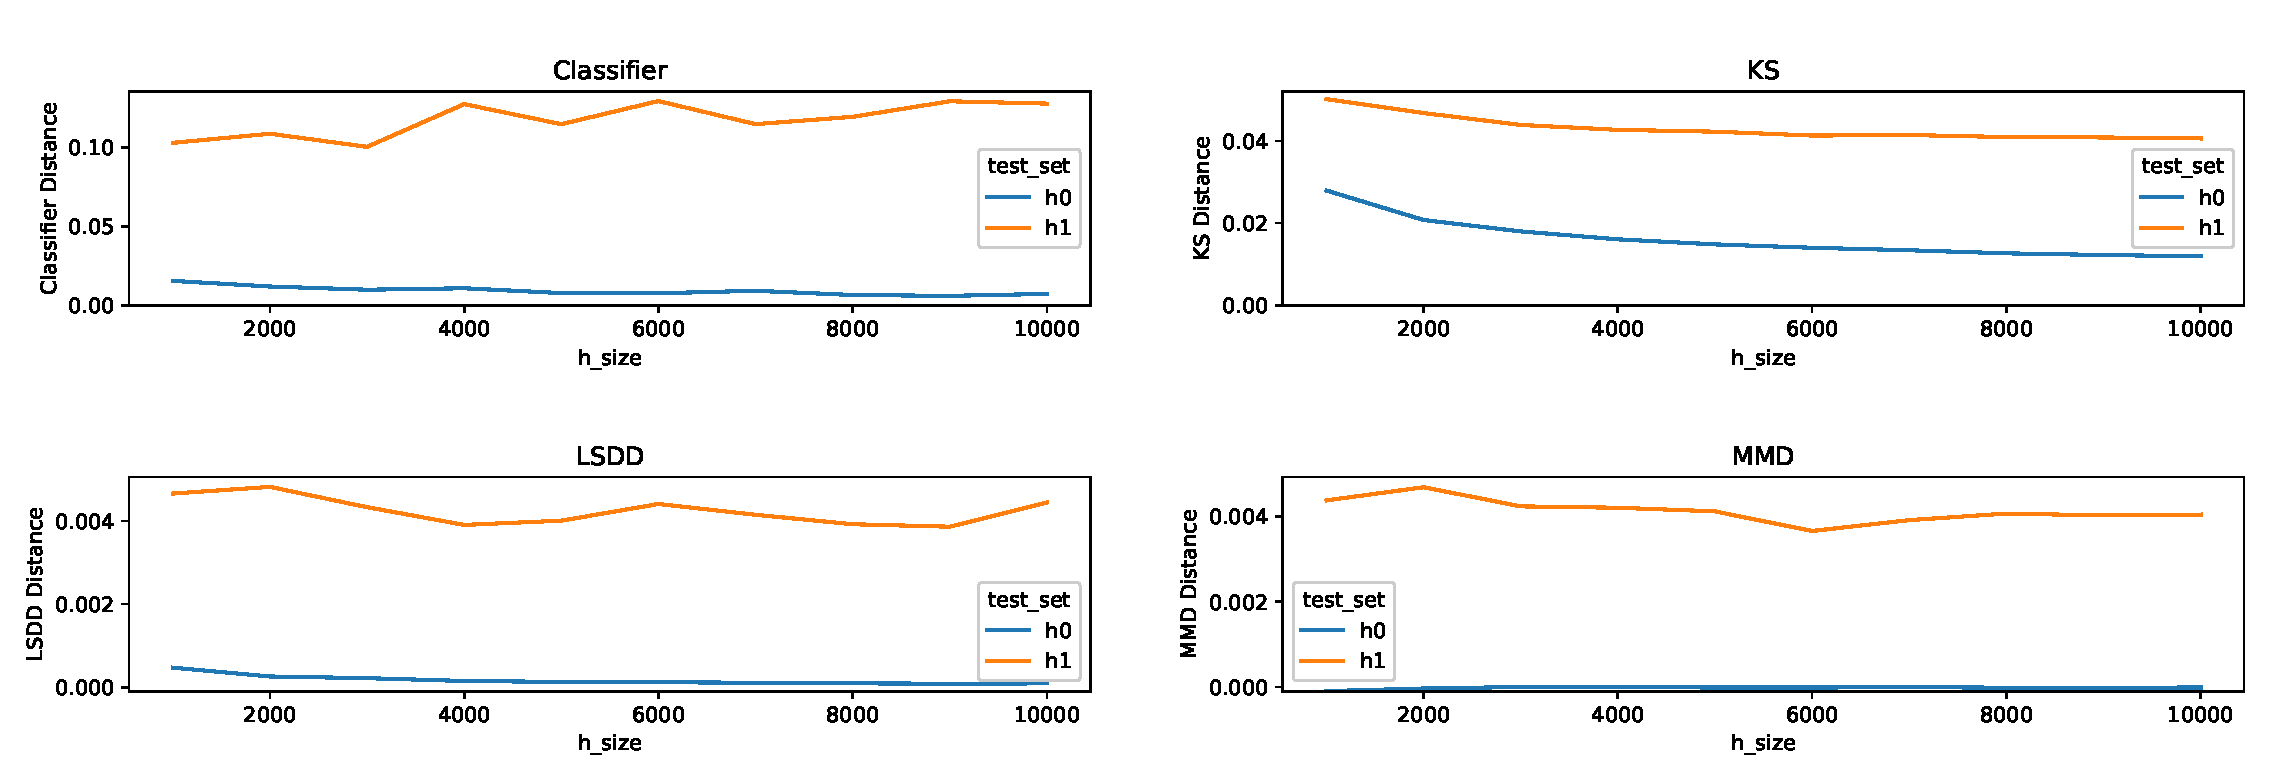
\includegraphics[width=\linewidth]{images/ALL-detector-distances}
\caption{Performance of the 4 detectors on different sizes of the test set, without (blue \(h_0\)) and with drift (orange \(h_1\)).}
\label{fig:distance}
\end{figure}

\section{Scalability}
We use the runtime to discuss what challenges we'll face when we will try to implement the methods in a production ML platform.
The runtime in our experiments is the time it takes to detect drift in different test data sizes.
\begin{itemize}
    \item It includes the distance calculation between \(p(x)\) and \(q(x')\).
    \item It includes the tokenization of \(DS_{test}\) to \(x_{h0}\) or \(x_{h1}\).
    \item The size of the reference distribution \(x_{ref}\) remains 10.000 samples across all runs.
    \item It does not include the loading of the LMs to the GPU memory.
    \item It does not include the loading of the text dataset to the CPU memory, nor the copy of the tensors to the GPU memory.
    \item In the case of KS, MMD and LSDD it does not include the time to tokenize the \(DS_{train}\) to \(x_{ref}\).
    \item In the case of the Classifier, the generation of \(x_{ref}\) is included, as we pass both datasets to the training process.
    \item The values shown are the average of the runtimes of 10 data points: 5 random splits for each of the undrifted \(h_0\) and the drifted test \(h_1\).
\end{itemize}

The selection of the test size is a key challenge in the detection of sequential changes, due to the false positive which can occur in the absence of change and the quadratic time of the MMD detector.
Cobb et al \cite{cobbSequentialMultivariateChange2021} propose a method for setting time-varying thresholds that allows a desired expected runtime to be accurately targeted whilst additionally keeping the false positive rate constant across time steps.

\begin{table}[h]
\begin{tabular}{|l|r|r|r|r|}
    \toprule
    detector &  Classifier &   KS &  LSDD &  MMD \\ \midrule
    h\_size &             &      &       &      \\ \midrule
    \midrule
    1000   &       146.5 & 13.1 &  13.1 & 25.6 \\ \midrule
    2000   &       165.0 & 16.6 &  14.6 & 31.2 \\ \midrule
    3000   &       177.0 & 16.9 &  15.0 & 33.9 \\ \midrule
    4000   &       184.4 & 16.6 &  18.3 & 38.9 \\ \midrule
    5000   &       198.7 & 19.5 &  17.2 & 42.9 \\ \midrule
    6000   &       212.8 & 19.0 &  20.4 & 47.6 \\ \midrule
    7000   &       231.9 & 21.5 &  19.7 & 51.7 \\ \midrule
    8000   &       243.3 & 21.5 &  21.6 & 58.9 \\ \midrule
    9000   &       254.7 & 25.4 &  22.1 & 62.8 \\ \midrule
    10000  &       264.4 & 25.4 &  22.9 & 69.9 \\ \midrule
    \bottomrule
\end{tabular}
\caption{Average runtime in seconds of the 4 detectors on different sizes of the test sets.}
\label{tab:runtime}
\end{table}

\subsection{Observations in the runtime}

\begin{itemize}
    \item All 4 methods have their runtime changing proportionally to the sample size of the test set.
    \item The Classifier has a penalty of time due to the nature of the algorithm: The reference set is given as input to a training process during the detection time, something that is not the case on the other methods.
    \item KS, LSDD and Classifier have a linear time computation complexity.
    \item MDD has log linear computation complexity, with worst case being quadratic due to the squared exponential kernel of the Gaussian RBF of the \(MMD^{2}\).
\end{itemize}

%observations

%* runtime changes proportionally to the test set size
%* drift detection effectiveness doesn't really change with the test set size

%* the choise of the test set size is very important


%* with fixed x size, as we increase the x':
%* for KS, LSDD, Classifier, the runtime scales in linear time
%* KS This comparison takes place only in the CPU memory so it has faster start up time without waiting to copy data to the gpu memory.
%* for MMD the runtime scale in log linear, with worst case being quadratic
%* due to the squared exponential kernel of the GaussianRBF in the mmd^2

%* All methods detect successfully the drifted from the original test sets
%* MMD detects h0 being part of the same distribution as ref quite close to 0

%* the caclulation time and amount of memory/cpu resources required
%* for the computation of drift, does not allow a cloud service to be provided
%* as value added but as a product. Essentially we're talking about running
%* a process during serving time, which is as computationally expensive as the
%* training


%The classifier outperforms the other detection methods in terms of


\begin{figure}[h]
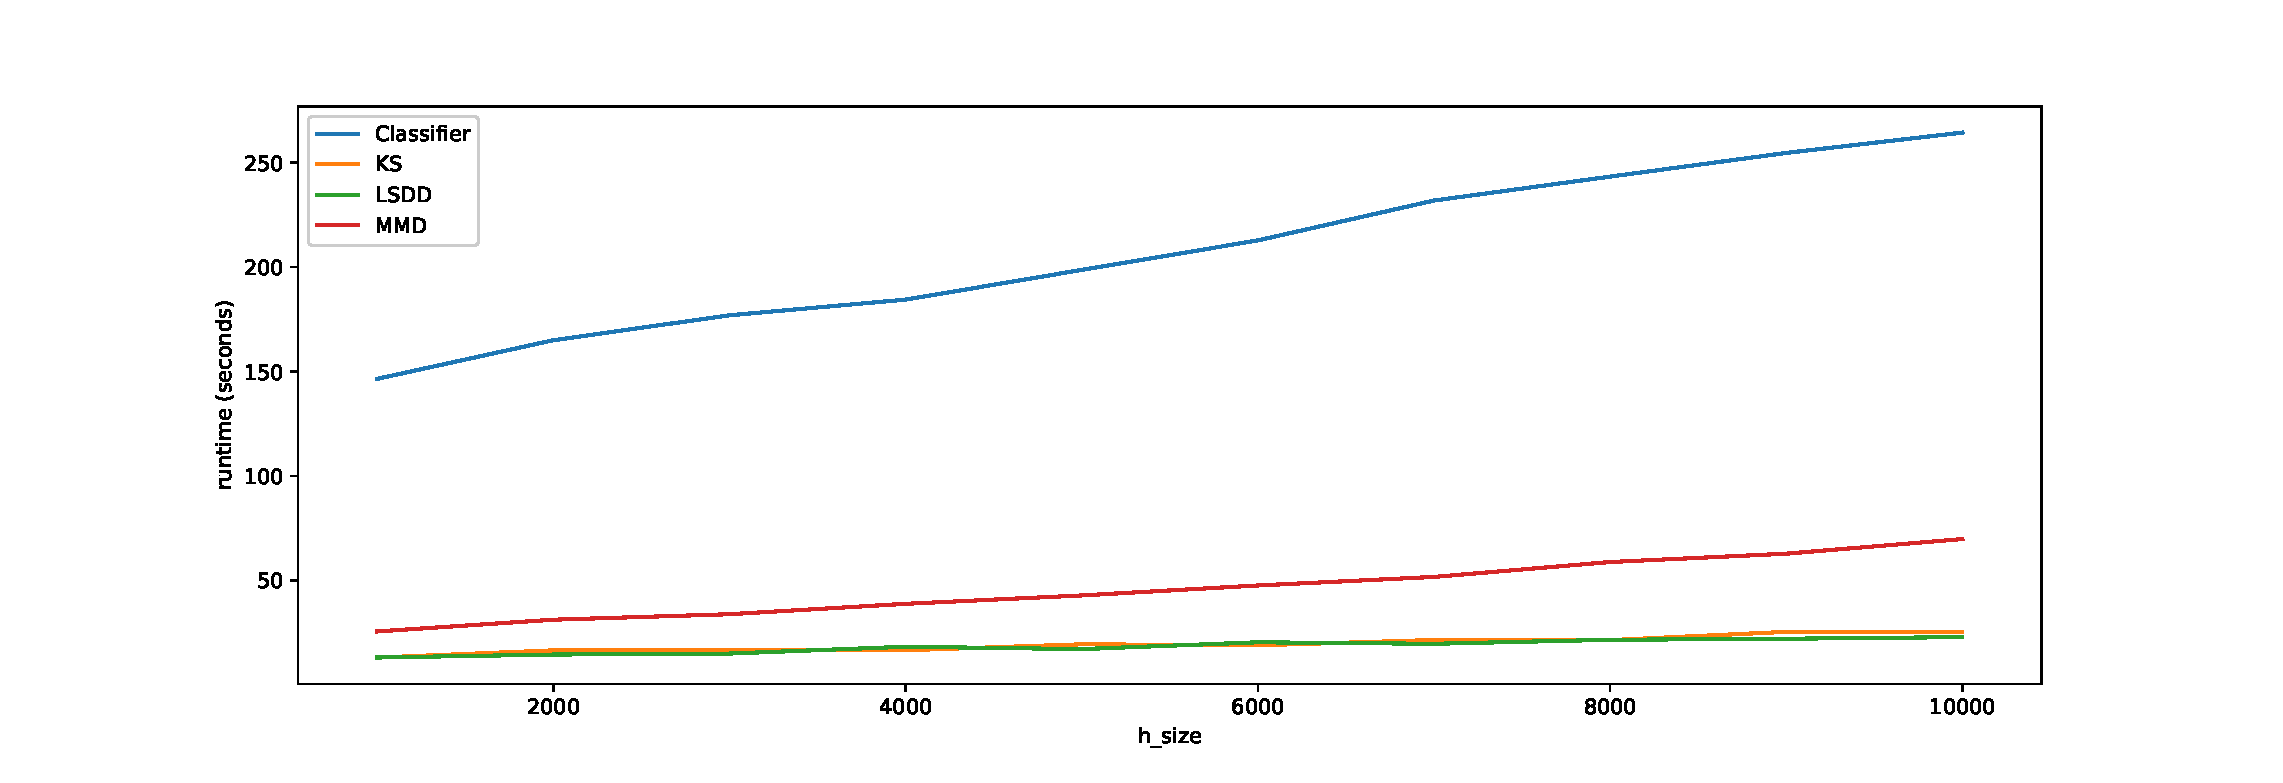
\includegraphics[width=\linewidth]{images/ALL-detectors-runtime}
\caption{Average runtime of the 4 detectors on different sample size of the test set.}
\label{fig:runtime}
\end{figure}

\begin{figure}[h]
    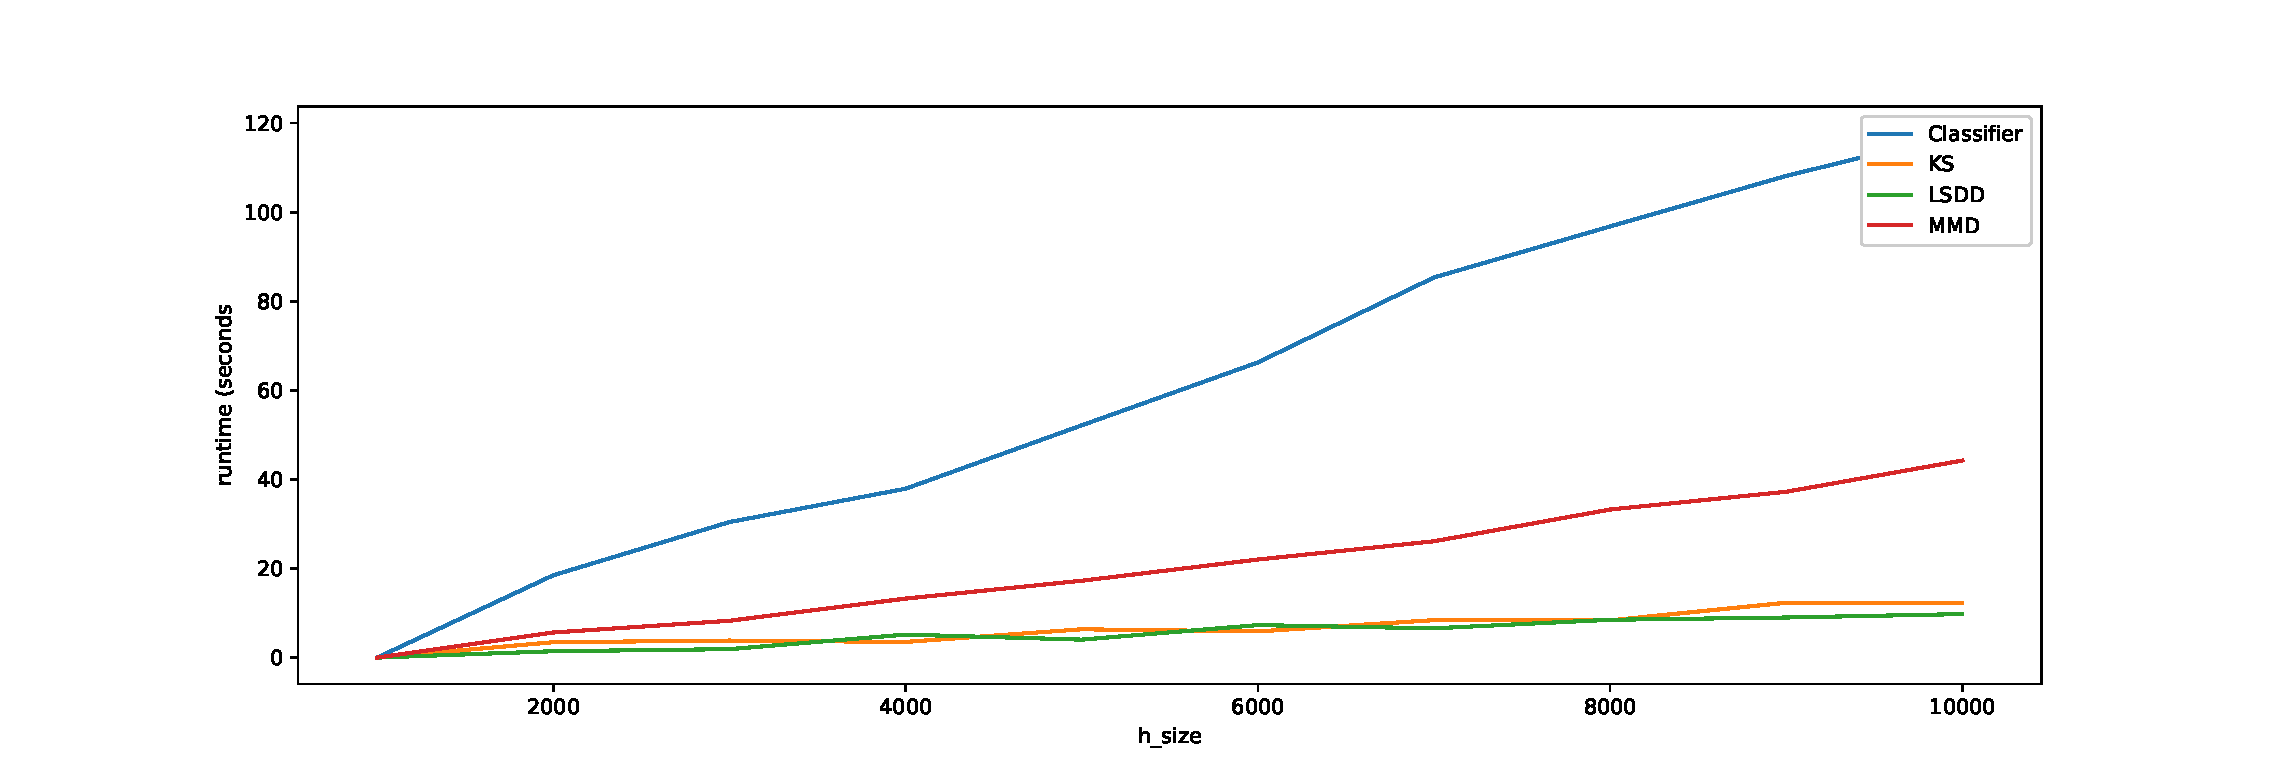
\includegraphics[width=\linewidth]{images/ALL-detectors-zeroed-runtime}
    \caption{Average runtime of the 4 detectors, positioned at the same starting point by subtracting the runtime of the first observation.}
    \label{fig:runtime_zeroed}
\end{figure}

%* drift introduction: filter by stars, filter by emotion
%* drift detection: KS, LSDD, MMD, Classifier
%* Classifier model: distilbert-base
%* KS: scipy ks_2samp
%* Across all detectors, the embeddings are calculated with the same model, and that time is included in the calculation.
%* seeds: different seeds of the random indeces for the dataset selection gave different metrics for everything else the same, so used 5 different seeds, commonly across the detector experiments
%* workflow: runner, worker, metrics, report
%* Tokenization: The text is passed to the bert model which returns the floats vector, the tensor is in the gpu memory.


%\chapter{Discussion}
%
% Univariate VS Multivariate Tests: We first evaluate whether we can detect shifts more easily using multiple univariate tests and aggregating their results via the Bonferroni correction or by using multivariate kernel tests. We were surprised to find that, despite the heavy correction, multiple univariate testing seem to offer comparable performance to multivariate testing (see Table 1a). Dimensionality Reduction Methods: For each testing method and experimental setting, we evaluate which DR technique is best suited to shift detection. Specifically in the multiple-univariatetesting case (and overall), BBSDs was the best-performing DR method. In the multivariate-testing case, UAE performed best. In both cases, these methods consistently outperformed others across sample sizes. The domain classifier, a popular shift detection approach, performs badly in the lowsample regime (≤ 100 samples), but catches up as more samples are obtained. Noticeably, the multivariate test performs poorly in the no reduction case, which is also regarded a widely used shift detection baseline. Table 1a summarizes these results. We note that BBSDs being the best overall method for detecting shift is good news for ML practitioners. When building black-box models with the main purpose of classification, said model can be Table 1: Dimensionality reduction methods (a) and shift-type (b) comparison. Underlined entries indicate accuracy values larger than 0.5. (a) Detection accuracy of different dimensionality reduction techniques across all simulated shifts on MNIST and CIFAR-10. Green bold entries indicate the best DR method at a given sample size, red italic the worst. Results for χ2 and Bin tests are only reported once under the univariate category. BBSDs performs best for univariate testing, while both UAE and TAE perform best for multivariate testing. Test DR Number of samples from test 10 20 50 100 200 500 1,000 10,000 Univ. tests NoRed 0.03 0.15 0.26 0.36 0.41 0.47 0.54 0.72 PCA 0.11 0.15 0.30 0.36 0.41 0.46 0.54 0.63 SRP 0.15 0.15 0.23 0.27 0.34 0.42 0.55 0.68 UAE 0.12 0.16 0.27 0.33 0.41 0.49 0.56 0.77 TAE 0.18 0.23 0.31 0.38 0.43 0.47 0.55 0.69 BBSDs 0.19 0.28 0.47 0.47 0.51 0.65 0.70 0.79 χ2 BBSDh 0.03 0.07 0.12 0.22 0.22 0.40 0.46 0.57 Bin Classif 0.01 0.03 0.11 0.21 0.28 0.42 0.51 0.67 Multiv. tests NoRed 0.14 0.15 0.22 0.28 0.32 0.44 0.55 PCA 0.15 0.18 0.33 0.38 0.40 0.46 0.55 SRP 0.12 0.18 0.23 0.31 0.31 0.44 0.54 UAE 0.20 0.27 0.40 0.43 0.45 0.53 0.61 TAE 0.18 0.26 0.37 0.38 0.45 0.52 0.59 BBSDs 0.16 0.20 0.25 0.35 0.35 0.47 0.50 (b) Detection accuracy of different shifts on MNIST and CIFAR-10 using the best-performing DR technique (univariate: BBSDs, multivariate: UAE). Green bold shifts are identified as harmless, red italic shifts as harmful. Test Shift Number of samples from test 10 20 50 100 200 500 1,000 10,000 Univariate BBSDs s gn 0.00 0.00 0.03 0.03 0.07 0.10 0.10 0.10 m gn 0.00 0.00 0.10 0.13 0.13 0.13 0.23 0.37 l gn 0.17 0.27 0.53 0.63 0.67 0.83 0.87 1.00 s img 0.00 0.00 0.23 0.30 0.40 0.63 0.70 0.93 m img 0.30 0.37 0.60 0.67 0.70 0.80 0.90 1.00 l img 0.30 0.50 0.70 0.70 0.77 0.87 0.97 1.00 adv 0.13 0.27 0.40 0.43 0.53 0.77 0.83 0.90 ko 0.00 0.00 0.07 0.07 0.07 0.33 0.40 0.70 m img+ko 0.13 0.40 0.87 0.93 0.90 1.00 1.00 1.00 oz+m img 0.67 1.00 1.00 1.00 1.00 1.00 1.00 1.00 Multivariate UAE s gn 0.03 0.03 0.03 0.03 0.03 0.07 0.07 m gn 0.03 0.03 0.03 0.03 0.17 0.27 0.30 l gn 0.50 0.57 0.67 0.70 0.80 0.90 1.00 s img 0.17 0.20 0.27 0.30 0.40 0.47 0.63 m img 0.23 0.33 0.37 0.40 0.47 0.60 0.70 l img 0.30 0.30 0.37 0.47 0.60 0.77 0.87 adv 0.03 0.20 0.27 0.27 0.33 0.40 0.40 ko 0.10 0.13 0.13 0.13 0.17 0.17 0.30 m img+ko 0.20 0.30 0.37 0.53 0.54 0.63 0.87 oz+m img 0.27 0.63 0.77 1.00 1.00 1.00 1.00 Table 2: Shift detection performance based on shift intensity (a) and perturbed sample percentages (b) using the best-performing DR technique (univariate: BBSDs, multivariate: UAE). Underlined entries indicate accuracy values larger than 0.5. (a) Detection accuracy of varying shift intensities. Test Intensity Number of samples from test 10 20 50 100 200 500 1,000 10,000 Univ. Small 0.00 0.00 0.14 0.14 0.18 0.36 0.40 0.54 Medium 0.14 0.21 0.39 0.38 0.42 0.57 0.66 0.76 Large 0.32 0.54 0.78 0.82 0.83 0.92 0.96 1.00 Multiv. Small 0.11 0.11 0.12 0.14 0.20 0.23 0.33 Medium 0.11 0.19 0.23 0.27 0.32 0.42 0.44 Large 0.34 0.45 0.57 0.68 0.72 0.82 0.93 (b) Detection accuracy of varying shift percentages. Test Percentage Number of samples from test 10 20 50 100 200 500 1,000 10,000 Univ. 10% 0.11 0.15 0.24 0.25 0.28 0.44 0.54 0.66 50% 0.14 0.28 0.52 0.53 0.60 0.68 0.72 0.85 100% 0.26 0.41 0.61 0.64 0.70 0.82 0.84 0.86 Multiv. 10% 0.12 0.13 0.21 0.26 0.27 0.31 0.44 50% 0.19 0.27 0.41 0.41 0.47 0.57 0.60 100% 0.29 0.41 0.44 0.53 0.60 0.70 0.78 easily extended to also double as a shift detector. Moreover, black-box models with soft predictions that were built and trained in the past can be turned into shift detectors retrospectively. Shift Types: Table 1b lists shift detection accuracy values for each distinct shift as an increasing amount of samples is obtained from the target domain. Specifically, we see that l gn, m gn, l img, m img+ko, oz+m img, and even adv are easily detectable, many of them even with few samples, while s gn, m gn, and ko are hard to detect even with many samples. With a few exceptions, the best DR technique (BBDSs for multiple univariate tests, UAE for multivariate tests) is significantly faster and more accurate at detecting shift than the average of all dimensionality reduction methods. Shift Strength: Based on the results in Table 2a, we can conclude that small shifts (s gn, s img, and ko) are harder to detect than medium shifts (m gn, m img, and adv) which in turn are harder to detect than large shifts (l gn, l img, m img+ko, and oz+m img). Specifically, we see that large shifts can on average already be detected with better than chance accuracy at only 20 samples using BBSDs, while medium and small shifts require orders of magnitude more samples in order to achieve similar accuracy. Moreover, the results in Table 2b show that while target data exhibiting only 10% anomalous samples are hard to detect, suggesting that this setting might be better addressed via outlier detection, perturbation percentages 50% and 100% can already be detected with better than chance accuracy using 50 samples. 101 102 103 104 Number of samples from test 0.0 0.2 0.4 0.6 0.8 1.0 p-value (a) Shift test (univ.) with 10% perturbed test data. 101 102 103 104 Number of samples from test 0.0 0.2 0.4 0.6 0.8 1.0 p-value (b) Shift test (univ.) with 50% perturbed test data. 101 102 103 104 Number of samples from test 0.0 0.2 0.4 0.6 0.8 1.0 p-value NoRed PCA SRP UAE TAE BBSDs BBSDh Classif (c) Shift test (univ.) with 100% perturbed test data. (d) Top different. 101 102 103 104 Number of samples from test 0.90 0.95 1.00 Accuracy (e) Classification accuracy on 10% perturbed data. 101 102 103 104 Number of samples from test 0.4 0.6 0.8 1.0 Accuracy (f) Classification accuracy on 50% perturbed data. 101 102 103 104 Number of samples from test 0.2 0.4 0.6 0.8 1.0 Accuracy p q Classif (g) Classification accuracy on 100% perturbed data. (h) Top similar. Figure 2: Shift detection results for medium image shift on MNIST. Subfigures (a)-(c) show the p-value evolution of the different DR methods with varying percentages of perturbed data, while subfigures (e)-(g) show the obtainable accuracies over the same perturbations. Subfigures (d) and (h) show the most different and most similar exemplars returned by the domain classifier across perturbation percentages. Plots show mean values obtained over 5 random runs with a 1-σ error-bar. 101 102 103 Number of samples from test 0.2 0.4 0.6 0.8 1.0 p-value (a) Shift test (univ.) with shuffled sets containing images from all angles. 101 102 103 Number of samples from test 0.0 0.2 0.4 0.6 0.8 1.0 p-value NoRed PCA SRP UAE TAE BBSDs BBSDh Classif (b) Shift test (univ.) with angle partitioned source and target sets. (c) Top different. 101 102 103 Number of samples from test 0.97 0.98 0.99 1.00 Accuracy (d) Classification accuracy on randomly shuffled sets containing images from all angles. 101 102 103 Number of samples from test 0.94 0.96 0.98 1.00 Accuracy p q Classif (e) Classification accuracy on angle partitioned source and target sets. (f) Top similar. Figure 3: Shift detection results on COIL-100 dataset. Subfigure organization is similar to Figure 2. Most Anomalous Samples and Shift Malignancy: Across all experiments, we observe that the most different and most similar examples returned by the domain classifier are useful in characterizing the shift. Furthermore, we can successfully distinguish malignant from benign shifts (as reported in Table 1b) by using the framework proposed in Section 3.4. While we recognize that having access to an external labeling function is a strong assumption and that accessing all true labels would be prohibitive at deployment, our experimental results also showed that, compared to the total sample size, two to three orders of magnitude fewer labeled examples suffice to obtain a good approximation of the (usually unknown) target accuracy. 0 5 10 15 20 25 0 5 10 15 20 25 Training set 6s — test set 6s -0.08 -0.06 -0.04 -0.02 0.00 0.02 0.04 0.06 0.08 0 5 10 15 20 25 0 5 10 15 20 25 Test set average for 6 0.0 0.1 0.2 0.3 0.4 0.5 0.6 0.7 0.8 0 5 10 15 20 25 0 5 10 15 20 25 Training set average for 6 0.0 0.1 0.2 0.3 0.4 0.5 0.6 0.7 0.8 Figure 4: Difference plot for training and test set sixes. Individual Examples: While full results with exact p-value evolution and anomalous samples are documented in the supplementary material, we briefly present two illustrative results in detail: (a) Synthetic medium image shift on MNIST (Figure 2): From subfigures (a)-(c), we see that most methods are able to detect the simulated shift with BBSDs being the quickest method for all tested perturbation percentages. We further observe in subfigures (e)-(g) that the (true) accuracy on samples from q increasingly deviates from the model’s performance on source data from p as more samples are perturbed. Since true target accuracy is usually unknown, we use the accuracy obtained on the top anomalous labeled instances returned by the domain classifier Classif. As we can see, these values significantly deviate from accuracies obtained on p, which is why we consider this shift harmful to the label classifier’s performance. (b) Rotation angle partitioning on COIL-100 (Figure 3): Subfigures (a) and (b) show that our testing framework correctly claims the randomly shuffled dataset containing images from all angles to not contain a shift, while it identifies the partitioned dataset to be noticeably different. However, as we can see from subfigure (e), this shift does not harm the classifier’s performance, meaning that the classifier can safely be deployed even when encountering this specific dataset shift. Original Splits: According to our tests, the original split from the MNIST dataset appears to exhibit a dataset shift. After inspecting the most anomalous samples returned by the domain classifier, we observed that many of these samples depicted the digit 6. A mean-difference plot (see Figure 4) between sixes from the training set and sixes from the test set revealed that the training instances are rotated slightly to the right, while the test samples are drawn more open and centered. To back up this claim even further, we also carried out a two-sample KS test between the two sets of sixes in the input space and found that the two sets can conclusively be regarded as different with a p-value of 2.7 · 10−10, significantly undercutting the respective Bonferroni threshold of 6.3 · 10−5. While this specific shift does not look particularly significant to the human eye (and is also declared harmless by our malignancy detector), this result however still shows that the original MNIST split is not i.i.d.

%observations

%* runtime changes proportionally to the test set size
%* drift detection effectiveness doesn't really change with the test set size

%* the choise of the test set size is very important


%* with fixed x size, as we increase the x':
%* for KS, LSDD, Classifier, the runtime scales in linear time
%* KS This comparison takes place only in the CPU memory so it has faster start up time without waiting to copy data to the gpu memory.
%* for MMD the runtime scale in log linear, with worst case being quadratic
%* due to the squared exponential kernel of the GaussianRBF in the mmd^2

%* All methods detect successfully the drifted from the original test sets
%* MMD detects h0 being part of the same distribution as ref quite close to 0

%* the caclulation time and amount of memory/cpu resources required
%* for the computation of drift, does not allow a cloud service to be provided
%* as value added but as a product. Essentially we're talking about running
%* a process during serving time, which is as computationally expensive as the
%* training


When a classifier is trained, we realize that we need much more processing resources than a typical inference service platform.
In the example of an inference serving platform, we have an ecosystem of peripheral services that are deployed around the model server, like the pre and postprocessing transformers, the explainers, the fairness detectors, the adversarial robustness testers, the logging and monitoring stack.
All these services are lightweight components compared to the core model server which usually requires a GPU instance to perform what it is meant to: the matrix multiplications between the weights of the model and the input vector of the inference request.
With the introduction of a drift detector, we are introducing two components: the drift detector itself and the epheneral storage for the test set.

The GPU instance type of the model server is optimized for inference, with accelerators like the AWS Elastic Inference which allocate a fraction of the VRAM to the model server.
The drift detector itself though, would require a GPU instance optimized for training, as it would need a larger amount of VRAM compared to the inference optimized resource allocation, to load the \(h_{ref}\) and \(h_0\) or \(h_1\) matrices.

On the topic of the ephemeral storage, the drift detector as a microservice requires as input a test dataset with multiple instances of incoming inference requests, unlike the explainers and transformers which consume single instances of inference requests from an event-based stream.
To achieve that, a model serving platform must be able to queue such a bucket of requests and bundle them to make them available to the detector.
The batch size of the test set is a critical parameter for the allocation of the resources to store such data.
Having a distributed streaming processing system would allow the detector to scale out to parallel, even overlapping tests, based on the batch size number or periods of time.
Such as system would handle the offsets of the detectors as consumers and essentially manage the scheduling of the tests.

Traditionally, a training pipeline delivers a model which is then loaded for inference in the model server.
In the case of the drift detector we have a second model (the detector's Classifier), sitting next to the model which performs the predictions for our product.
It also means that we have a continuous training pipeline, which also refreshes the \(x_{ref}\) periodically or based on a trigger.
The traditional data pipeline scheduler are not the best options for such a scenario, and a ml pipeline solution would be optimal \cite{baylorContinuousTrainingProduction2019} for data-driven execution of the pipeline.

%The classifier outperforms the other detection methods in terms of

\chapter{Conclusion}

% In this paper, we put forth a comprehensive empirical investigation, examining the ways in which dimensionality reduction and two-sample testing might be combined to produce a practical pipeline for detecting distribution shift in real-life machine learning systems. Our results yielded the surprising insights that (i) black-box shift detection with soft predictions works well across a wide variety of shifts, even when some of its underlying assumptions do not hold; (ii) that aggregated univariate tests performed separately on each latent dimension offer comparable shift detection performance to multivariate two-sample tests; and (iii) that harnessing predictions from domain-discriminating classifiers enables characterization of a shift’s type and its malignancy. Moreover, we produced the surprising observation that the MNIST dataset, despite ostensibly representing a random split, exhibits a significant (although not worrisome) distribution shift. Our work suggests several open questions that might offer promising paths for future work, including (i) shift detection for online data, which would require us to account for and exploit the high degree of correlation between adjacent time steps [22]; and, since we have mostly explored a standard image classification setting for our experiments, (ii) applying our framework to other machine learning domains such as natural language processing or graphs.

%https://docs.seldon.io/projects/alibi-detect/en/stable/overview/algorithms.html
% spot-the-diff
% classifier uncertainty
% regressors uncertainty

%\cite{schrouffMaintainingFairnessDistribution2022} explore the settings in which recently proposed mitigation strategies are applicable by referring to a causal framing


The Classifier method outperforms MMD and other baseline methods like KS and LSDD.
It also makes easier the frequently change of \(h_{ref}\) as it's loading it every time together with the \(h_{ref}\).
It comes with a penalty of extra time required for training the classifier with the reference and test dataset.

Implementing a monitoring solution for a ML platform in the space of drift detection brings two important challenges: the selection of the test set size and the allocation of computation resources.
The test size can be empirically defined based on the number of samples or a time period.
Recent research \cite{cobbSequentialMultivariateChange2021} \cite{kublerAutoMLTwoSampleTest2022} is trying to automate such detection configuration.
The scaling of the resources for the drift detector should be handled by a platform that is capable of managing the batches of the inference requests in a data-driven fashion.


%\bibliographystyle{plain}
%\bibliography{bibentries}
\printbibliography

\end{document}

